% Data read from the bar labels of arXiv:2406.09324v3 (Xu, Liu, and Liu, 2024),
% Figures 4 (safety system prompt) and 5 (chat template), AutoDAN and PAIR panels.
% Values are unchanged; the charts are redrawn in pgfplots.
\definecolor{xubase}{RGB}{140,140,140}
\definecolor{xutest}{RGB}{35,103,159}
\pgfplotsset{
  xubars/.style={
    ybar, bar width=14pt, width=\linewidth, height=4.6cm,
    ymin=0, ymax=105, ytick={0,20,...,100},
    symbolic x coords={Llama-2-7B,Llama-3-8B,Vicuna-7B,Qwen1.5-7B,Mistral-7B},
    xtick=data, enlarge x limits=0.11, axis lines=box,
    grid=major, grid style={black!12},
    tick label style={font=\scriptsize}, label style={font=\footnotesize},
    title style={font=\bfseries\small}, ylabel={ASR (\%)},
    nodes near coords, nodes near coords align={vertical},
    every node near coord/.append style={font=\tiny, /pgf/number format/fixed},
    legend style={font=\scriptsize, at={(0.5,-0.2)}, anchor=north, legend columns=-1, draw=none, /tikz/every even column/.append style={column sep=8pt}},
    area legend,
  }
}
\newcommand{\xupanel}[5]{% title, legend A, legend B, data A, data B
  \begin{axis}[xubars, title={#1}]
    \addplot[draw=xubase!80!black, fill=xubase!55] coordinates {#4};
    \addplot[draw=xutest!80!black, fill=xutest!60] coordinates {#5};
    \legend{#2, #3}
  \end{axis}}

\begin{figure}[htbp]
\centering
\caption[Safety system prompts in Xu et al.]{Attack success rate (ASR) of AutoDAN and PAIR attacks on five open-weight models, without (grey) and with (blue) a safety system prompt (ssp). ASR is the cited benchmark's binary attack-success metric, not this dissertation's graded StrongREJECT outcome.}
\label{fig:xu-system-prompts}
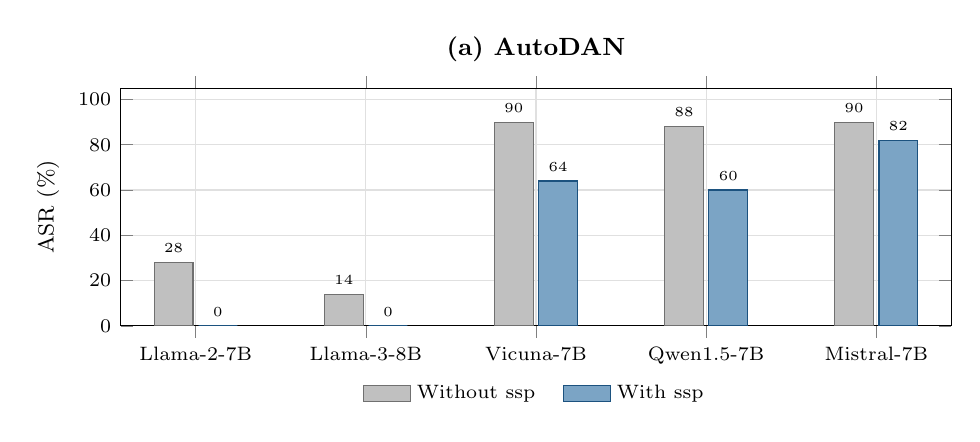
\begin{tikzpicture}
  \xupanel{(a) AutoDAN}{Without ssp}{With ssp}
    {(Llama-2-7B,28) (Llama-3-8B,14) (Vicuna-7B,90) (Qwen1.5-7B,88) (Mistral-7B,90)}
    {(Llama-2-7B,0) (Llama-3-8B,0) (Vicuna-7B,64) (Qwen1.5-7B,60) (Mistral-7B,82)}
\end{tikzpicture}

\medskip
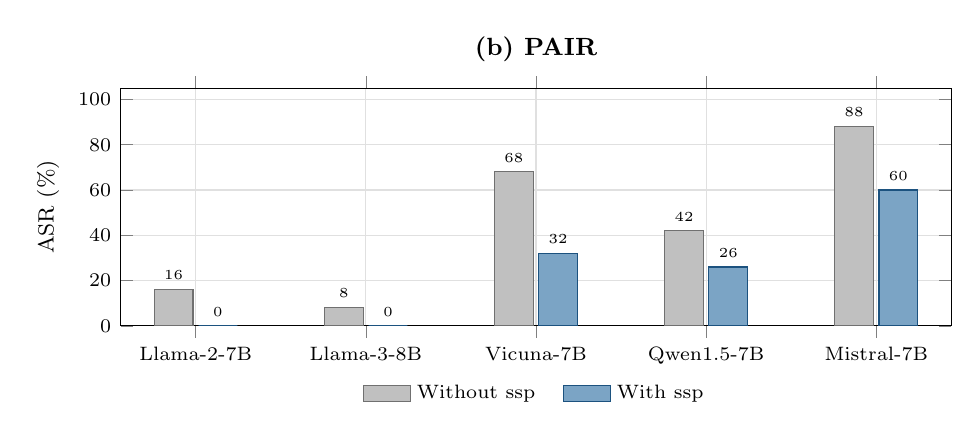
\begin{tikzpicture}
  \xupanel{(b) PAIR}{Without ssp}{With ssp}
    {(Llama-2-7B,16) (Llama-3-8B,8) (Vicuna-7B,68) (Qwen1.5-7B,42) (Mistral-7B,88)}
    {(Llama-2-7B,0) (Llama-3-8B,0) (Vicuna-7B,32) (Qwen1.5-7B,26) (Mistral-7B,60)}
\end{tikzpicture}
\fonte{Adapted from \textcite{xuBagTricksBenchmarking2024}.}
\end{figure}

\begin{figure}[htbp]
\centering
\caption[Chat-template comparison in Xu et al.]{Attack success rate (ASR) of AutoDAN and PAIR attacks on five open-weight models under a zero-shot chat template (grey) and the model's default template (blue). These external benchmark results motivate controlling prompt format; they do not estimate a template effect in this dissertation.}
\label{fig:xu-chat-templates}
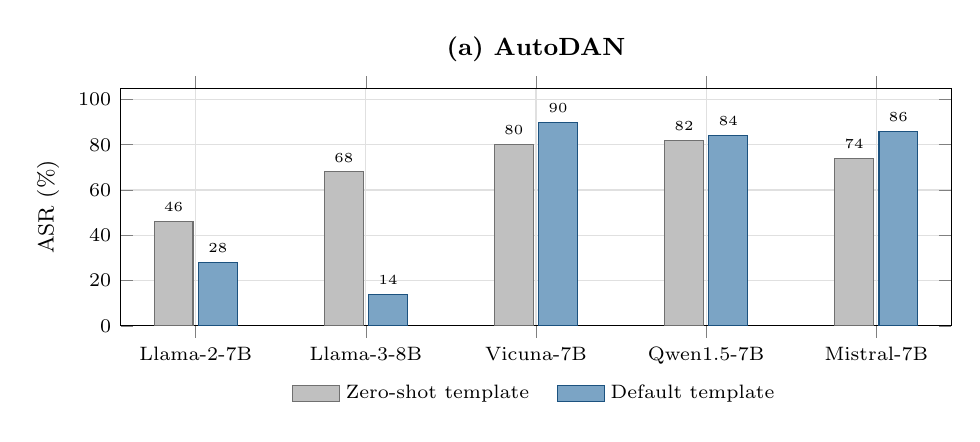
\begin{tikzpicture}
  \xupanel{(a) AutoDAN}{Zero-shot template}{Default template}
    {(Llama-2-7B,46) (Llama-3-8B,68) (Vicuna-7B,80) (Qwen1.5-7B,82) (Mistral-7B,74)}
    {(Llama-2-7B,28) (Llama-3-8B,14) (Vicuna-7B,90) (Qwen1.5-7B,84) (Mistral-7B,86)}
\end{tikzpicture}

\medskip
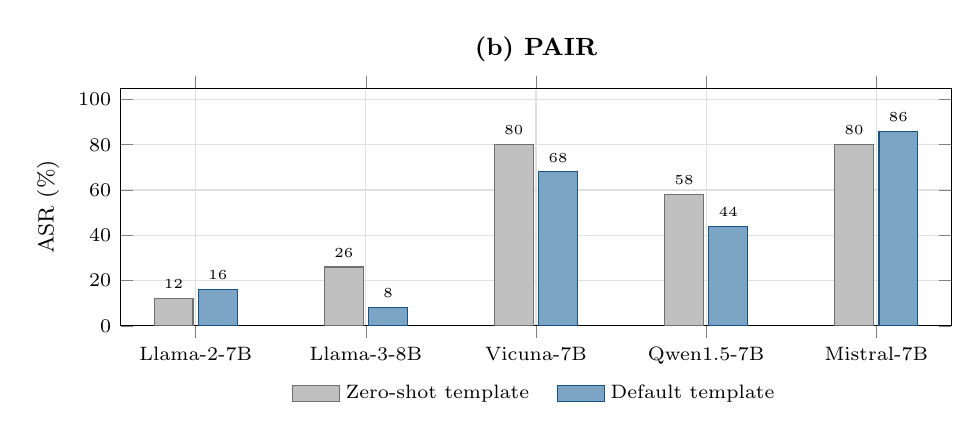
\begin{tikzpicture}
  \xupanel{(b) PAIR}{Zero-shot template}{Default template}
    {(Llama-2-7B,12) (Llama-3-8B,26) (Vicuna-7B,80) (Qwen1.5-7B,58) (Mistral-7B,80)}
    {(Llama-2-7B,16) (Llama-3-8B,8) (Vicuna-7B,68) (Qwen1.5-7B,44) (Mistral-7B,86)}
\end{tikzpicture}
\fonte{Adapted from \textcite{xuBagTricksBenchmarking2024}.}
\end{figure}
